\documentclass{article}

\usepackage[utf8]{inputenc}
\usepackage[left=2.5cm, right=2.5cm, top=2.5cm, bottom=2.5cm]{geometry}
\usepackage{amsmath}
\usepackage{authblk}
\usepackage{bm}
\usepackage[labelfont=bf, textfont=it]{caption}
\usepackage{csquotes}
\usepackage{graphicx}
\usepackage{natbib}
\usepackage{subcaption}
\usepackage{url}
\usepackage{xcolor}




\title{Bayesian Estimation and Forecasting of Internal Migration Rates: An Application to England}

\author[1]{Junni L. Zhang}
\author[2]{John Bryant}

\affil[1]{China Center for Economic Research, National School of Development and Center for Statistical Science, Peking University, Beijing, China}
\affil[2]{Bayesian Demography Limited, Christchurch, New Zealand}


\date{}

\begin{document}


\maketitle
  
\begin{abstract}
Internal migration is a key driver of subnational population trends. Modeling and forecasting internal migration rates is, however, technically challenging, due to the heterogeneity of regional age-sex patterns and the sparsity of the data. In this paper, we show how Bayesian hierarchical models can accommodate this heterogeneity and sparsity. We apply three increasingly complex models to data on internal migration in the United Kingdom during the period 2012--2024. We use Bayesian model selection and model checking techniques to choose between the three models. We then use the selected model to forecast detailed internal migration rates over the period 2025--2030.

\end{abstract}

\noindent \textbf{Keywords:} direct estimate, age profile, interaction, small area estimation, Bayesian hierarhical model, model selection

%\pagenumbering{gobble} 

%\newpage

%\pagenumbering{gobble} 


%\newpage

\section{Introduction}

Forecasting future population size and age-sex structure at sub-national levels is essential for effective regional planning of schools, hospitals, and housing \citep{wilson2015short, zhang2020bayesian}. Internal migration is a key driver of population change at sub-national levels, and sometimes outweighing births and deaths in shaping local demographic trends \citep{deschermeier2011population}. Internal migration can also drive disparities in labor markets and economic development \citep{rees2019role}.

Internal migration rates measure migration intensities, that is, how frequently people move relative to the population at risk. Unlike raw counts of migrants, rates are standardized, making them comparable across regions and time periods with different population sizes and different age-sex structures. This comparability allows researchers and planners to identify whether migration behavior is truly changing, which is a prerequisite for designing internal migration policies. For instance, policies to retain young adults in a depopulating region might reflect an elevated out‑migration rate rather than solely by a large number of leavers, which may simply reflect the region's large population size. Internal migration rates can also be embedded in formal demographic models to forecast future population size and age-sex structure at sub-national levels \citep[e.g.][]{willekens1978spatial}.

It is not easy to identify which features of historical trends in internal migration rates can safely be extrapolated into the future, since the heterogeneity across sub-national areas can be substantial. For instance, the age profiles of migrants coming to university towns are drastically different from those of migrants coming to rural areas \citep{wilson2010model}. When internal migration is finely disaggregated, e.g., by age, sex, region of origin and region of destination, heterogeneity is even more prominent. Furthermore, in some cases the numbers of observations for some combinations of the classifying variables can be small, and individual-level randomness starts to obscure underlying patterns. Traditional `direct' estimates of rates, obtained by dividing observed migration counts by populations at risk, are no longer reliable \citep{zhang2020bayesian}.

One way to extract complex signals from {\color{yellow}sparse,} noisy datasets is to use Bayesian hierarchical models \citep{Gelman2014bayesian}. These models allow analysts to encode expectations about the qualitative behaviour of model components, through the use of prior distributions, and also to borrow strength across subgroups within the population, to cope with sparsity. Bayesian hierarchical models have been increasingly popular among researchers carrying out sub-national demographic estimation and forecasting \citep{lynch2010obtaining,schmertmann2013bayes,bijak2016bayesian,alexander2017flexible,bryant2018bayesian,wang2022spatiotemporal,alexander2022bayesian,dharamshi2025jointly,omenti2026bayesian}. 

There is a limited literature on Bayesian methods for modelling and forecasting internal migration \citep{wisniowski2014baysian,zhang2020bayesian,furfaro2021bayesian,goes2026probabilistic}. {\color{magenta}\cite{siriban2026review}, 
\cite{goes2026probabilistic} ***}


{\color{magenta}After more than a decade of effort, we have developed a flexible Bayesian hierarchical modeling framework for estimating and forecasting disaggregated demographic rates. We have also developed flexible and computationally efficient software for fitting, checking, and using these models. In this paper, we apply the framework to estimate internal migration rates in England from 2012 to 2024, disaggregated by single year of age, sex, and origin and destination region. Within this framework, we specify several models of increasing complexity. }
{\color{yellow}In this paper, we develop several Bayesian models that can capture complex patterns in internal migration, and apply them to estimate internal migration rates for the period 2012–2024 for the UK, disaggregated by single year of age, sex, region of origin and region of destination.} We perform model selection and model checking, and then use the selected model to forecast internal migration rates over the period 2025–2030. {\color{magenta}Almost all computations are carried out using our software.}{\color{yellow}An important part of our efficient computation builds on the ideas in \cite{liu2001monte}, and in particular on the collapsed Gibbs sampling in \cite{liu1994collapsed}.}

The remaining parts of the paper are organized as follows. Section 2 presents the UK internal migration data and patterns in the data. Section 3 discusses several Bayesian models and covers the computation. Section 4 then turns to model selection and model checking. Section 5 presents results on estimation and forecasting. Section 6 then concludes. All data and computer code for the analysis are available at [url for GitHub repository].

\section{Data}\label{sec:data}
Our data consist of counts of internal migration and population size by single year of age (up to age 90+), sex, region of origin, region of destination, and calendar year for the period 2012–2024. The data were obtained from the Office for National Statistics website \citep{ons2025internalmigration,ons2025population}{\color{magenta}; detailed internal migration data are available only for 2012–2024}. There are 9 regions {\color{magenta} in England}: London, East of England (shortened to ``E"), North East (``NE"), North West (``NW"), South East (``SE"), South West (``SW"), East Midlands (``EM"), West Midlands (``WM"), and Yorkshire and The Humber (``YH"). 
{\color{magenta}Figure~\ref{fig:map_england} shows a map of these regions.}
 \begin{figure}[htp]
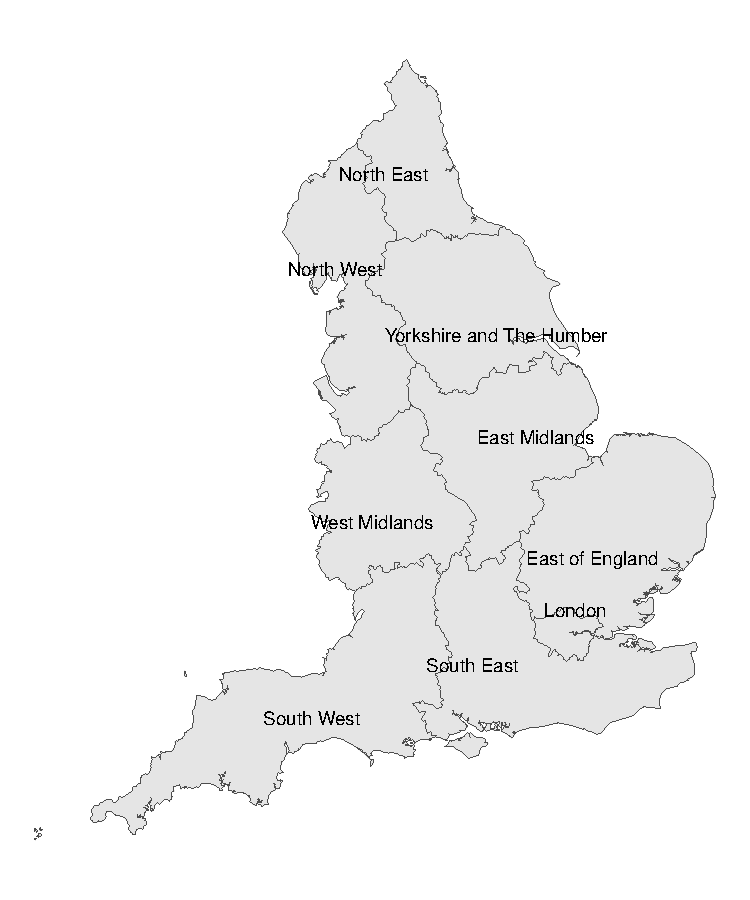
\includegraphics[width = 0.5\textwidth]{figures/fig_map_england}
  \centering
  \caption{The regions of England. Source: \citet{ons2024regions}.}
    \label{fig:map_england}  
\end{figure}

Since internal migration requires a change of region, region of destination cannot equal region of origin. Altogether, there are 170,352 (91$\times$2$\times$9$\times$8$\times$13) cells. Population at risk is generally large, with a minimum value of 1,749 and a maximum value of 91,340.
{\color{yellow}The data on internal migration counts show some sparsity.}{\color{magenta}The internal migration count data contain many low counts.} There are 1,562 cells (0.9\%) with internal migration counts equal to zero, and 25,350 cells (14.9\%) with internal migration counts below 10.

\begin{figure}[htp]
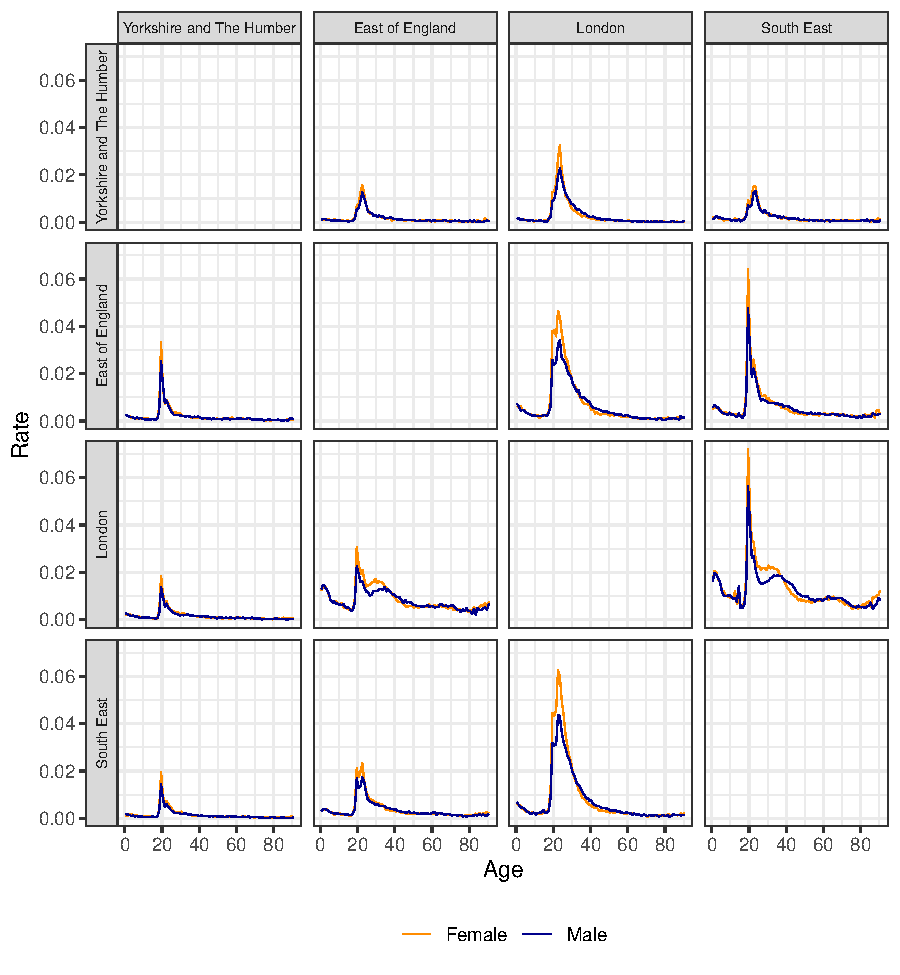
\includegraphics[width = \textwidth]{figures/fig_direct_age_2016}
  \centering
  \caption{Direct estimates of migration rates, by region of origin, region of destination, age and sex for selected regions in 2016. Each row represents one origin region and each column represents one destination region.}\label{fig:direct_2016}  \end{figure}
  
Figure~\ref{fig:direct_2016} displays direct estimates of migration rates by region of origin, region of destination, age, and sex for selected regions in 2016. The age profiles show dramatic differences across origin-destination pairs. For instance, migration from other regions to London peaks at age 22–23, whereas migration from London to other regions peaks at age 19. The sharp spikes around age 19 mainly reflect migration for tertiary education. Migration from London to the South East shows an increase at the highest ages, whereas migration from London to Yorkshire and the Humber does not have this pattern. There is also heterogeneity in age profiles between females and males across origin-destination pairs. For instance, between ages 19 and 25, migration rates from the East of England to London are higher for females than for males. However, there is only a slight difference in the age profiles between females and males for migration from the East of England to Yorkshire and the Humber.

\begin{figure}[htp]
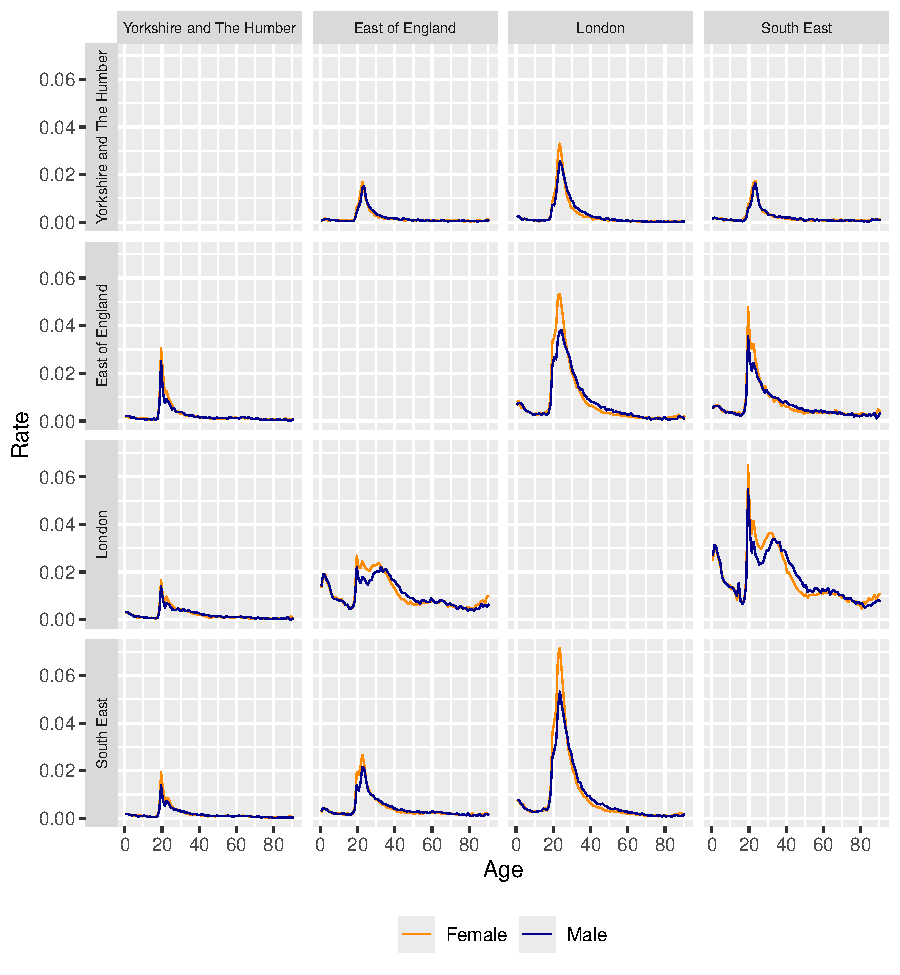
\includegraphics[width = \textwidth]{figures/fig_direct_age_2021}
  \centering
  \caption{Direct estimates of migration rates, by region of origin, region of destination, age and sex for selected regions in 2021. Each row represents one origin region and each column represents one destination region.}\label{fig:direct_2021}  \end{figure}

Figure~\ref{fig:direct_2021} displays information similar to that in Figure~\ref{fig:direct_2016}, but for year 2021. The age profiles again show dramatic differences across origin-destination pairs. For the same origin-destination pairs, the age profiles also change across time. For instance, for migration from London to the South East in 2016, the peak rate at age 19 is much larger than the rates at ages 25–35, but this gap becomes smaller in 2021.

Figure~\ref{fig:summary_direct} displays direct estimates of migration rates by region of origin, region of destination, sex, and calendar year for selected regions, for which migration counts and population at risk have been aggregated over age. The effect of the COVID-19 pandemic is visible in most of the series, with a dip in migration during 2020 and a surge in migration during the years that followed. However, there is heterogeneity in time trends across origin-destination pairs. For example, migration rates from London to the East of England show the following trend: slow increase, then flat, then a sharp increase followed by a sharp decrease, then flat again. Migration from London to the South East follows a similar pattern, but with greater fluctuations. Migration rates from London to Yorkshire and the Humber, however, remain almost flat throughout the entire period. 

{\color{magenta}As shown in Figure~\ref{fig:map_england}, the East of England and the South East are the two regions neighboring London. As \citet{Lange2024} points out, the shift to working from home has weakened ties to the office, and gardens and access to the outdoors have become higher priorities. Such shifts in preferences may help explain the migration patterns described above.}

There is only a small difference in time trends between sexes for some origin-destination pairs.

 \begin{figure}[htp]
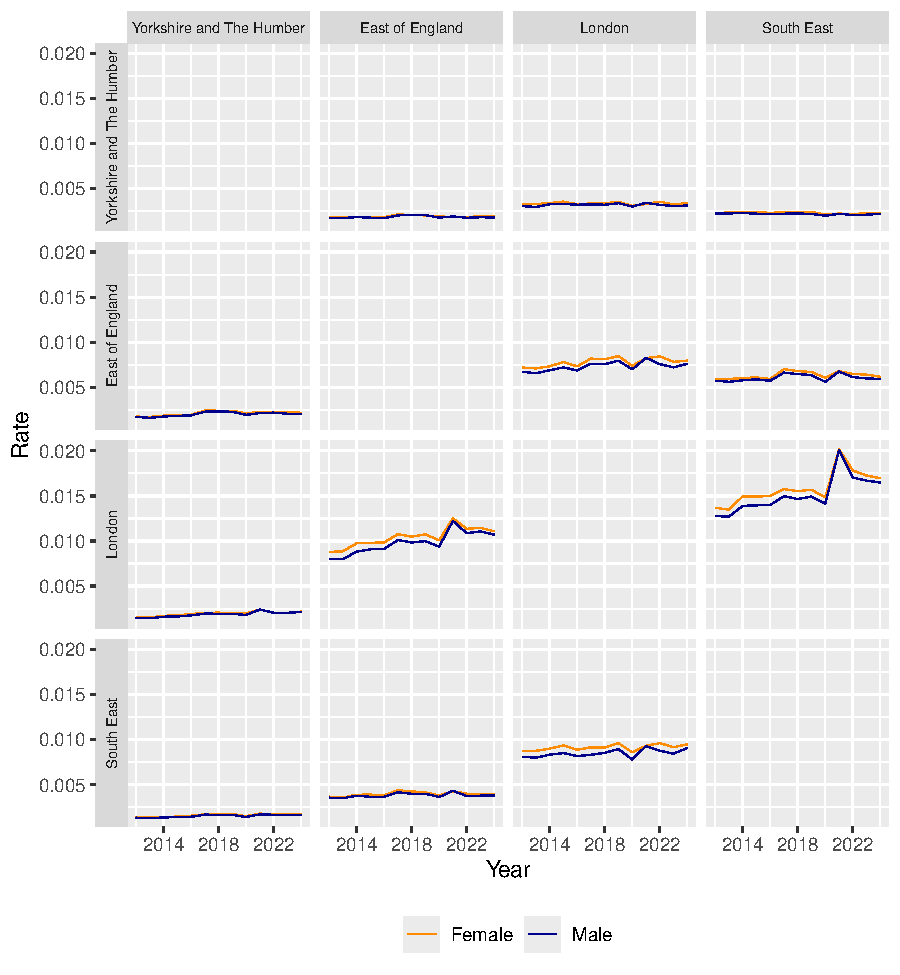
\includegraphics[width = \textwidth]{figures/fig_direct_time}
  \centering
  \caption{Direct estimates of migration rates, by region of origin, region of destination, and calendar year for selected regions. Each row represents one origin region and each column represents one destination region.}\label{fig:summary_direct}   
%\vspace{1ex}
%\newline\small\scriptsize{\textsf{\textit{Note}:  The results shown here are a more complete version of results shown in Figure 6 in the main text.}}
\end{figure}

\section{Bayesian Models and Computation}\label{sec:models}

\subsection{{\color{yellow}Baseline Model}{\color{magenta}Initial Model}}

\subsubsection{Counts and Rates}
Let $y_{ijast}$ denote migration counts from region $i$ ($i=1,\cdots,9$) to region $j$ ($j=1,\cdots,9$ and $j\neq i$) for age group $a$ ($a=1$ for age 0, $\cdots$, $a=91$ for age $90+$) and sex $s$ ($s=1$ for females and $s=0$ for males) during year $t$
($t=1$ for 2012, $\cdots$, $t=13$ for 2024). Let $P_{iast}$ denote the population at risk for region $i$, age group $a$, sex $s$ in year $t$. We assume that{\color{yellow}, within each cell, migration counts} {\color{magenta}migration counts are independent across cells and that each migration count} follow a Poisson distribution,
\begin{equation}
y_{ijast}\sim\text{Poisson}(\gamma_{ijast}P_{iast}),\label{eq:poisson}
\end{equation}
where $\gamma_{ijast}$ is the underlying migration rate.

{\color{magenta}This implies that, for a given origin–age–sex–year combination, the destination-specific migration counts are independent Poisson random variables with the same population at risk. This is equivalent to specifying a Poisson distribution for the total migration count from each origin–age–sex–year combination and then, conditional on this total, specifying a multinomial distribution for the counts across competing destinations.}

We model $\gamma_{ijast}$ as a draw from a Gamma distribution, with expectation governed by $\mu_{ijast}$ and dispersion governed by $\xi$,
\begin{equation}
 \gamma_{ijast} \sim \text{Gamma}(\xi^{-1}, (\xi \mu_{ijast})^{-1}). \label{eq:priormod1}
\end{equation}
\noindent Parameter $\xi$ is equivalent to a ``flexibility parameter'' in a penalized complexity prior \citep{simpson2017penalising}, in that larger values imply a more flexible model with larger departures from expected value $\mu_{ijast}$. We assign $\xi$ an exponential prior, with rate 1, which favors small values for $\xi$.

The posterior mean for $\gamma_{ijast}$, conditional on $y_{ijast}$, $w_{ijast}$, $\mu_{ijast}$, and $\xi$, can be written as
\begin{equation}
    \hat{\gamma}_{ijast} = \lambda_{ijast} \frac{y_{ijast}}{w_{ijast}} + (1 - \lambda_{ijast}) \mu_{ijast}
\end{equation}
where
\begin{equation}
    \lambda_{ijast} = \frac{\mu_{ijast} w_{ijast}}{\xi^{-1} + \mu_{ijast} w_{ijast}}.
\end{equation}
The posterior mean is a weighted average of a cell-specific direct estimate of migration rate $y_{ijast}/w_{ijast}$ and a prior mean $\mu_{ijast}$. The prior mean receives more weight as the amount of information for the cell, represented by expected count $\mu_{ijast} w_{ijast}$, falls. The estimate for any given cell borrows strength, via the prior model, from all cells in the model. This leads to more stable estimates than direct estimates. 

\subsubsection{Priors}\label{subsec:priors}
The prior model relates the expected rate to terms reflecting variation across region of origin, region of destination, age, sex, and time,
\begin{equation}
\begin{aligned}
 \log \mu_{ijast} &= \beta^0 + \beta_i^{\text{orig}}+\beta_j^{\text{dest}}+\beta_{a}^{\text{age}}+\beta_{s}^{\text{sex}}+\beta_t^{time} \\
 & + \beta_{ia}^{\text{orig:age}}+ \beta_{ja}^{\text{dest:age}}+\beta_{as}^{\text{age:sex}}+\beta_{at}^{\text{age:time}}+ \beta_{ij}^{\text{orig:dest}}\\
 &+\beta_{it}^{\text{orig:time}}+\beta_{jt}^{\text{dest:time}}.  
\end{aligned}\label{eq:priormod2}    
\end{equation}
In \eqref{eq:priormod2}, $\beta^0$ is an intercept term; $\beta_i^{\text{orig}}$, $\beta_j^{\text{dest}}$, $\beta_a^{\text{age}}$, $\beta_s^{\text{sex}}$ and $\beta_t^{\text{time}}$ are main effects for region of origin, region of destination, age, sex and time;    $\beta_{ia}^{\text{orig:age}}$, $\beta_{ja}^{\text{dest:age}}$, $\beta_{as}^{\text{age:sex}}$, $\beta_{at}^{\text{age:time}}$,
$\beta_{ij}^{\text{orig:dest}}$,
$\beta_{it}^{\text{orig:time}}$ and $\beta_{jt}^{\text{dest:time}}$ are interaction terms capturing origin-age, destination-age, age-sex, age-time, origin-destination, origin-time and destination-time interactions. 

As shown in Section \ref{sec:data}, 
age profiles change across region of origin, region of destination, sex and time, so we have included interactions between age and each of the other dimensions; 
there is a great deal of variation across origin‑destination pairs, so we have included an origin‑destination interaction; there is also evidence for different time trends across origin-destination pairs, so we have included origin-time and destination-time interactions.

The prior for the intercept is a standard normal distribution,
$\beta^0\sim N(0,1)$. Since $\beta^0$ is common to all cells,  the information from the data will dominate the prior.

The prior for the origin effect, $\beta_i^{\text{orig}}$, is a normal distribution,
\begin{equation}
\beta_i^{\text{orig}}\sim N(0,\sigma_{\text{orig}}^2).
\end{equation}
The standard deviation parameter $\sigma_{\text{orig}}$ is shared across all regions.  {\color{magenta}It needs a prior itself. Here and elsewhere in the model we use weakly informative priors that set orders of magnitude rather than narrowly constraining results \citep[p. 55]{Gelman2014bayesian}. We assign $\sigma_{\text{orig}}$}
{\color{yellow}, and is given} a half-normal prior
$\sigma_{\text{orig}}\sim N^+(0,1).$ 
The prior for the destination effect, $\beta_j^{\text{dest}}$, is similar.

The prior for the age effects, $\beta_a^{\text{age}}$, is a second order random walk (RW2),
\begin{equation}
\begin{aligned}
\beta_1^{\text{age}}&{\color{yellow}=0}{\color{magenta}\sim N(0,1)},\\
\beta_2^{\text{age}}&\sim N(0,1),\\
\beta_a^{\text{age}}&\sim N(2\beta_{a-1}^{\text{age}}-\beta_{a-2}^{\text{age}},\sigma_{\text{age}}^2),\ a=3,\cdots,A,
\end{aligned}
\end{equation}
where $A=91$ is the number of age groups.
The standard deviation parameter $\sigma_{\text{age}}$ is given a half-normal prior $\sigma_{\text{age}}\sim N(0,1).$

The second-order random walk model was originally developed for modeling change over time. It implies a locally linear trend, where the slope  follows a random walk. This makes it suitable for time series where the underlying trend changes unpredictably. However, it works equally well for modeling change over age. As we can see from Section~\ref{sec:data}, age effects can also change unpredictably. {\color{yellow}Setting $\beta_1^{\text{age}}=0$ helps with identification.}

The prior for the sex effect, $\beta_s^{\text{sex}}$, is a standard normal distribution, $\beta_s^{\text{sex}}\sim N(0,1)$.

The prior for the time effect $\beta_t^{\text{time}}$ consists of a linear trend $\alpha_t^{\text{time}}$ and a second-order autoregressive (AR2) residual  $\kappa_t^{\text{time}}$,
\begin{equation}
\begin{aligned}
\beta_t^{\text{time}}&=\alpha_t^{\text{time}}+\kappa_t^{\text{time}},\\
\alpha_t^{\text{time}}&=\left(t-\frac{T+1}{2}\right) \eta^{\text{time}},\\
\kappa_t^{\text{time}}&\sim N(\phi_1\kappa_{t-1}^{\text{time}}+\phi_2\kappa_{t-2}^{\text{time}},\sigma_{\text{time}}^2),
\end{aligned}
\end{equation}
where $T=13$ is the number of years in the observed data. The trend terms sum to zero, $\sum_{t=1}^T\alpha_t^{\text{time}}=0$. The use of an AR2 prior for errors around the trend can capture reversion to the mean, but is also flexible enough to represent other patterns of errors. 

The parameters in the prior for the time effect themselves need priors. {\color{yellow}Here and elsewhere in the model we use weakly informative priors that set orders of magnitude rather than narrowly constraining results \citep[p. 55]{Gelman2014bayesian}.} The value of the standard deviation $\sigma_{\text{time}}$ in the AR2 prior is chosen so that each $\kappa_t^{\text{time}}$ has marginal distribution $\text{N}(0, \varphi_{\text{time}}^2)$, where 
$\varphi_{\text{time}} \sim \text{N}^+(0,1)$. Values for $\kappa_1^{\mathcal{T}}$ and $\kappa_2^{\mathcal{T}}$ are generated through the Yule-Walker equations, which is the standard way of generating initial conditions in an auto-regressive process (\citealp[pp.~45--46]{prado2021time}; \citealp{tmb2025ar}). We use the prior
\begin{equation}
  \frac{\phi_k + 1}{2} \sim \text{Beta}(5, 5), \quad k = 1, 2
\end{equation}
for the autoregressive coefficients. This prior restricts the coefficients to values between -1 and 1, and discourages values that are very close to the boundaries, which helps prevent numerical problems. {\color{magenta}The construction of the marginal variance and the initialization via the Yule–Walker equations require the AR2 prior to be stationary. Since $-1<\phi_2<1$ is already ensured, the remaining stationarity conditions are $\phi_1+\phi_2<1$ and $\phi_2-\phi_1<1$. Although we do not impose these remaining restrictions a priori, we check the posterior draws of $\phi_1$ and $\phi_2$ and find that they satisfied these conditions.}

The prior for the origin-age interaction effect, $\beta_{ia}^{\text{orig:age}}$, is a region-specific first order random walk over age,
\begin{equation}
\begin{aligned}
\beta_{i1}^{\text{orig:age}}&{\color{yellow}=0}{\color{magenta}\sim N(0,1)},\\
\beta_{ia}^{\text{orig:age}}&\sim N(\beta_{i,a-1}^{\text{orig:age}},\sigma_{\text{orig:age}}^2),\ a=2,\cdots,A.
\end{aligned}
\end{equation}
The standard deviation parameter $\sigma_{\text{orig:age}}$ is shared across all regions, and is given a half-normal prior $\sigma_{\text{orig:age}}\sim N^+(0,1)$. The prior for the destination-age interaction effect, $\beta_{ja}^{\text{dest:age}}$, is similar.

The prior for the age-sex interaction effect, $\beta_{as}^{\text{age:sex}}$, is a sex-specific first-order random walk over age,
\begin{equation}
\begin{aligned}
\beta_{1s}^{\text{age:sex}}&{\color{yellow}=0}{\color{magenta}\sim N(0,1)},\\
\beta_{as}^{\text{age:sex}}&\sim N(\beta_{a-1,s}^{\text{age:sex}},\sigma_{\text{age:sex}}^2),\ a=2,\cdots,A.
\end{aligned}
\end{equation}
The standard deviation parameter $\sigma_{\text{age:sex}}$ is shared across both sexes, and is given a half-normal prior $\sigma_{\text{age:sex}}\sim N^+(0,1)$.

The prior for the age-time interaction effect, $\beta_{at}^{\text{age:time}}$, is an age-specific first order random walk over time, \begin{equation}
\begin{aligned}
\beta_{a1}^{\text{age:time}}&{\color{yellow}=0}{\color{magenta}\sim N(0,1)},\\
\beta_{at}^{\text{age:time}}&\sim N(\beta_{a,t-1}^{\text{age:time}},\sigma_{\text{age:time}}^2),\ t=2,\cdots,T.
\end{aligned}
\end{equation}
The standard deviation parameter $\sigma_{\text{age:time}}$ is shared across all ages, and is given a half-normal prior $\sigma_{\text{age:time}}\sim N^+(0,1)$.

The prior for the origin-destination interaction effect, $\beta_{ij}^{\text{orig:dest}}$, is a normal distribution,
\begin{equation}
\beta_{ij}^{\text{orig:dest}}\sim N(0,\sigma_{\text{orig:dest}}^2).
\end{equation}
The standard deviation parameter $\sigma_{\text{orig:dest}}$ is shared across all origin-destination pairs, and is given a half-normal prior $\sigma_{\text{orig:dest}}\sim N^+(0,1)$.

The prior for the origin-time interaction effect, $\beta_{it}^{\text{orig:time}}$, is a region-specific first order random walk over time,
\begin{equation}
\begin{aligned}
\beta_{i1}^{\text{orig:time}}&{\color{yellow}=0}{\color{magenta}\sim N(0,1)},\\
\beta_{it}^{\text{orig:time}}&\sim N(\beta_{i,t-1}^{\text{orig:time}},\sigma_{\text{orig:time}}^2),\ t=2,\cdots,T.
\end{aligned}
\end{equation}
The standard deviation parameter $\sigma_{\text{orig:time}}$ is shared across all regions, and is given a half-normal prior $\sigma_{\text{orig:time}}\sim N^+(0,1)$. The prior for the destination-time interaction effect, $\beta_{jt}^{\text{dest:time}}$, is similar.

Table \ref{tab:prior-summary} summarizes the priors for terms in the {\color{yellow}baseline}{\color{magenta}initial} model.
\begin{table}[ht]
\centering
\caption{Summary of priors for terms in the baseline model}
\label{tab:prior-summary} 
\begin{tabular}{l p{9cm}}
  \hline
Term & Specification \\ 
  \hline
Intercept & Standard normal\\
Origin & Normal with a half-normally distributed standard deviation\\
Destination & Normal with a half-normally distributed standard deviation\\
Age & Second-order random walk\\
Sex & Standard normal\\
Time & Linear trend with second-order autoregressive error term \\
Origin-age & Region-specific first order random walks over age\\
Destination-age & Region-specific first order random walks over age\\
  Age-sex & Sex-specific first-order random walks over age\\
  Age-time & Age-specific first-order random walks over time \\
  Origin-Destination & Normal with a half-normally distributed standard deviation\\
  Origin-time & Region-specific first order random walks over time\\
  Destination-time & Region-specific first order random walks over time\\
  \hline
\end{tabular}
\end{table}

\subsection{Two Expanded Models}
As shown in Figures~\ref{fig:direct_2016} and ~\ref{fig:direct_2021}, the age profile of migration rate can be drastically different across origin-destination pairs. Including only origin-age and destination-age interactions may not be sufficient. Therefore we also consider an expanded model with a three-way origin-destination-age interaction effect, $\beta_{ija}^{\text{orig:dest:age}}$. 

The prior for the origin-destination-age interaction effect, $\beta_{ija}^{\text{orig:dest:age}}$, is an origin-destination pair-specific first-order random walk over age,
\begin{equation}
\begin{aligned}
\beta_{ij1}^{\text{orig:dest:age}}&{\color{yellow}=0}{\color{magenta}\sim N(0,1)},\\
\beta_{ija}^{\text{orig:dest:age}}&\sim N(\beta_{i,j,a-1}^{\text{orig:dest:age}},\sigma_{\text{orig:dest:age}}^2),\ a=2,\cdots,A.
\end{aligned}
\end{equation}
The standard deviation parameter $\sigma_{\text{orig:dest:age}}$ is shared across all origin-destination pairs, and is given a half-normal prior $\sigma_{\text{orig:dest:age}}\sim N^+(0,1)$. 

To further capture the higher-order interaction between age, origin, destination, sex and time, we specify another expanded model with two additional four-way interaction effects: origin-destination-age-sex and origin-destination-age-time interactions. 

The prior for the origin-destination-age-sex interaction effect, $\beta_{ijas}^{\text{orig:dest:age:sex}}$, is an origin-destination-sex-specific first-order random walk over age,
\begin{equation}
\begin{aligned}
\beta_{ij1s}^{\text{orig:dest:age:sex}}&{\color{yellow}=0}{\color{magenta}\sim N(0,1)},\\
\beta_{ijas}^{\text{orig:dest:age:sex}}&\sim N(\beta_{i,j,a-1,s}^{\text{orig:dest:age:sex}},\sigma_{\text{orig:dest:age:sex}}^2),\ a=2,\cdots,A.
\end{aligned}
\end{equation}
The standard deviation parameter $\sigma_{\text{orig:dest:age:sex}}$ is shared across all origin-destination-sex triples, and is given a half-normal prior $\sigma_{\text{orig:dest:age:sex}}\sim N^+(0,1)$. 

The prior for the origin-destination-age-time interaction effect, $\beta_{ijas}^{\text{orig:dest:age:time}}$, is an origin-destination-age-specific first-order random walk over time,
\begin{equation}
\begin{aligned}
\beta_{ija1}^{\text{orig:dest:age:time}}&{\color{yellow}=0}{\color{magenta}\sim N(0,1)},\\
\beta_{ijat}^{\text{orig:dest:age:time}}&\sim N(\beta_{i,j,a,t-1}^{\text{orig:dest:age:time}},\sigma_{\text{orig:dest:age:time}}^2),\ a=2,\cdots,A.
\end{aligned}
\end{equation}
The standard deviation parameter $\sigma_{\text{orig:dest:age:time}}$ is shared across all origin-destination-age triples, and is given a half-normal prior $\sigma_{\text{orig:dest:age:time}}\sim N^+(0,1)$. 

\subsection{{\color{magenta}Main Effects Model}}
{\color{magenta}As a simple baseline for comparison, we also specify a model with only main effects and no interactions:
\begin{equation*}
\begin{aligned}
 \log \mu_{ijast} &= \beta^0 + \beta_i^{\text{orig}}+\beta_j^{\text{dest}}+\beta_{a}^{\text{age}}+\beta_{s}^{\text{sex}}+\beta_t^{time}.
\end{aligned}
\end{equation*}
The priors for the main effects are the same as those in the previous three models.}

\subsection{{\color{magenta}Model Identification and Regularization}}

{\color{magenta}All four models contain a large number of parameters. Each involves 170,352 cell-specific migration rates ($\gamma_{ijast}$) and the dispersion parameter $\xi$. The main effects model has 125 $\beta$ parameters (e.g., $\beta^0$, $\beta_i^{\text{orig}}$) and 7 hyper-parameters (e.g., $\sigma_{\text{orig}}$); the initial model has 3,443 $\beta$ parameters and 27 hyper-parameters (e.g., $\sigma_{\text{orig}}$, $\kappa_t^{\text{time}}$); the first expanded model has 10,814 $\beta$ parameters and 28 hyper-parameters; and the second expanded model has 121,379 $\beta$ parameters and 30 hyper-parameters.}

{\color{magenta}The expected rates $\mu_{ijast}$ are determined by the $\beta$ parameters. Note that the Gamma prior for 
$\gamma_{ijast}$ conditional on $\mu_{ijast}$ in \eqref{eq:priormod1} is conjugate to the Poisson likelihood for $y_{ijast}$ conditional on $\gamma_{ijast}$ in \eqref{eq:poisson}. Consequently, integrating out $\gamma_{ijast}$ yields the negative binomial distribution
\begin{equation}\label{eq:negbinom}
  y_{ijast} \sim \text{NegBinom}\left(\xi^{-1}, (1 + \mu_{ijast} P_{iast} \xi)^{-1}\right),
\end{equation}
as in \citep{norton2018sampling}. Thus, we can generate posterior draws of the $\beta$ parameters and hyper-parameters and then, conditional on these draws, generate posterior draws of $\gamma_{ijast}$ in a post-processing step, using
\begin{equation}\label{eq:generate_gamma}
  \gamma_{ijast} \mid y_{ijast}, P_{iast}, \mu_{ijast}, \xi \sim \text{Gamma}\left(y_{ijast} + \xi^{-1}, P_{iast} + (\xi \mu_{ijast})^{-1}\right).
\end{equation}
This is analogous to the marginalization strategy used in collapsed Gibbs sampling \citep{liu1994collapsed}.}

{\color{magenta}Even after marginalizing over $\gamma_{ijast}$, the initial model and the two expanded models still contain a large number of $\beta$ parameters. We do not perform sparse shrinkage or selection of interactions in the usual sense (e.g., spike-and-slab variable selection in \cite{george1993variable} or horseshoe shrinkage in \cite{carvalho2010horseshoe}). Instead, the roughness and magnitude of the specified interactions are controlled through hierarchical priors. Proper priors ensure a proper posterior. However, since the observed migration counts $y_{ijast}$ depend on the expected rates $\mu_{ijast}$  that are linear combinations of the $\beta$ parameters,  identification of the individual $\beta$ parameters may be weak.  Fortunately, we are interested in the rates $\gamma_{ijast}$ which depend on $\mu_{ijast}$, rather than in the individual $\beta$ parameters per se. 
} 

\subsection{Computation}

We fit the model using our own R package \texttt{bage}. The package implements {\color{yellow}a general family of Bayesian hierarchical models}{\color{magenta}the flexible Bayesian hierarchical modeling framework that we have developed}. Users can specify the likelihood (Poisson, Binomial, or Normal), the main and interaction terms to include, and the priors for each of these terms.

The \texttt{bage} package draws on the R package \texttt{TMB} \citep{kristensen2016tmb} to estimate the $\beta$ parameters {\color{yellow}(e.g., $\beta^0$, $\beta_i^{\text{orig}}$)} and their hyper-parameters {\color{yellow}(e.g., $\sigma_{\text{orig}}$, $\kappa_t^{\text{time}}$)}, as well as the dispersion parameter 
$\xi$. \texttt{TMB} combines a Laplace approximation and numerical integration \citep{kristensen2016tmb,osgood2022statistical}. {\color{magenta}In the Laplace approximation, we maximize the log marginal posterior density with respect to the $\beta$ parameters, the hyperparameters, and $\xi$, with the standard deviation parameters on the log scale. We then generate draws of the $\beta$ parameters, the hyperparameters and $\xi$ from a multivariate normal distribution, again with the standard deviation parameters on the log scale.}{\color{yellow}Borrowing the idea of collapsed Gibbs sampling from \cite{liu1994collapsed}, we marginalize out the rates $\gamma_{ijast}$ during model fitting. This dramatically reduces the dimension of the problem, which further increases computational speed and allows us to avoid using Laplace approximations for these quantities.} We {\color{yellow}derive values for}{\color{magenta}obtain draws of} $\gamma_{ijast}$ in a post-processing step{\color{magenta}, as in \eqref{eq:generate_gamma}}. {\color{yellow}Details are provided in the Appendix.} 

{\color{magenta}The Laplace approximation underlying \texttt{TMB} belongs to a broader class of approximate Bayesian inference methods that have been shown to be reliable and computationally efficient. \citet{rue2017bayesian} use integrated nested Laplace approximations (INLA) to perform approximate Bayesian inference for latent Gaussian models (LGMs), a class that includes a large proportion of the statistical models used today. They show that INLA (and the associated \texttt{R-INLA} package) performs inference within a reasonable time frame and in most cases is both faster and more accurate than MCMC alternatives. \citet{osgood2023statistical} provide a large-scale simulation study that assesses and compares \texttt{R-INLA} and \texttt{TMB} for continuous spatial models, and find that the predictive fields from both methods are comparable in most situations. We have used our package \texttt{bage} (which builds on \texttt{TMB}) for many demographic estimation and forecasting problems and find the results satisfactory, as assessed by posterior predictive checks and held-out data validation.}

{\color{cyan}John. Referee 1's comments: The reported runtimes are useful, but computational reporting could also be made more informative by specifying the exact processor, number of cores/threads, whether parallelization is used, peak memory consumption, and whether the reported times include generation of the posterior draws. Because computational scalability is emphasized as an advantage of the approach, even a limited empirical assessment of scaling with the number of cells and/or model
  terms would be valuable.} These times are relatively fast, given the number of parameters being estimated. {\color{yellow}All three models have 170,352 rate parameters ($\gamma_{ijast}$) and the dispersion parameter $\xi$. The baseline model has 3,443 $\beta$ parameters  and 27 hyper-parameters, the first expanded model has 10,814 $\beta$ parameters and 28 hyper-parameters, and the second expanded model has 121,379 $\beta$ parameters and 30 hyper-parameters.}

% latex table generated in R 4.6.1 by xtable 1.8-8 package
% Fri Oct 30 14:01:51 2026
\begin{table}[ht]
\centering
\caption{Resources used for model fitting} 
\label{tab:resources}
\begin{tabular}{lcc}
  \hline
Model & Elapsed time (seconds) & Peak memory usage (GiB) \\ 
  \hline
Initial & 218 & 7.8 \\ 
  First expanded & 423 & 8.3 \\ 
  Second expanded & 1531 & 8.0 \\ 
   \hline
\end{tabular}
\end{table}


\section{Model Selection and Model Checking}

\subsection{WAIC}

To perform model selection among the baseline model and the expanded models, we use
 the Watanabe-Akaike or Widely Applicable Information Criterion (WAIC) \citep{watanabe2010asymptotic}. As pointed out by Section 7.2 of \cite{Gelman2014bayesian}, compared to other information criteria that condition on a point estimate, WAIC has the desirable property of averaging over the posterior distribution, which is more compatible with Bayesian model selection.

{\color{yellow}Let the posterior samples of $\gamma_{ijast}$ be $\{\gamma_{ijast}^{(r)}:\ r=1,\cdots,R\}$. Let $$p\left(y_{ijast}|\gamma_{ijast}^{(r)}w_{ijast}\right)$$ be the probability of $y_{ijast}$ in a Poisson distribution with rate $\gamma_{ijast}^{(r)}w_{ijast}$. We first obtain the computed log pointwise predictive density as
\begin{equation}
\text{computed}\ lppd=\sum_{i,j,a,s,t}\log\left(\frac{1}{R}\sum_{r=1}^R p\left(y_{ijast}|\gamma_{ijast}^{(r)}w_{ijast}\right)\right).
\end{equation}
This quantity measures the fit between the model and the data.
Next, let $Var_{r=1}^R \left(\log p\left(y_{ijast}|\gamma_{ijast}^{(r)}w_{ijast}\right)\right)$ denote the posterior sample variance of the log predictive density for each data point $y_{ijast}$. The effective number of parameters is 
\begin{equation}
\text{computed}\ p_{WAIC}=\sum_{i,j,a,s,t}Var_{r=1}^R \left(\log p\left(y_{ijast}|\gamma_{ijast}^{(r)}w_{ijast}\right)\right).
\end{equation}}

{\color{magenta}We are interested in forecasting migration rates, and the expected rates $\mu_{ijast}$ for future years and the dispersion parameter $\xi$ are relevant to forecasting. To align with this forecasting objective, we calculate the WAIC conditional on the expected rates $\mu_{ijast}$ for historical years and $\xi$.}

{\color{magenta}Let the posterior draws of $\mu_{ijast}$ for historical years be $\{\mu_{ijast}^{(r)}:\ r=1,\cdots,R\}$. Let $$p\left(y_{ijast}|P_{ijast},\mu_{ijast}^{(r)},\xi\right)$$ be the probability of $y_{ijast}$ under the negative binomial distribution given in \eqref{eq:negbinom}, conditional on $P_{ijast}$, $\mu_{ijast}^{(r)}$ and $\xi$. We first obtain the computed log pointwise predictive density as
\begin{equation}
\text{computed}\ lppd=\sum_{i,j,a,s,t}\log\left(\frac{1}{R}\sum_{r=1}^R p\left(y_{ijast}|P_{ijast},\mu_{ijast}^{(r)},\xi\right)\right).
\end{equation}
This quantity measures the fit between the model and the data.
Next, let $Var_{r=1}^R \left(\log p\left(y_{ijast}|P_{ijast},\mu_{ijast}^{(r)},\xi\right)\right)$ denote the posterior sample variance of the log predictive density for each data point $y_{ijast}$. The effective number of parameters is 
\begin{equation}
\text{computed}\ p_{WAIC}=\sum_{i,j,a,s,t}Var_{r=1}^R \left(\log p\left(y_{ijast}|P_{ijast},\mu_{ijast}^{(r)},\xi\right)\right).
\end{equation}}
This quantity measures the complexity of the model. The WAIC represents a tradeoff between model fit and model complexity, and equals 
\begin{equation}
WAIC=-2(\text{computed}\ lppd-\text{computed}\ p_{WAIC}).
\end{equation}
{\color{yellow}We select the model with the smaller WAIC.} {\color{magenta}The model with the smallest WAIC is preferred.}

% latex table generated in R 4.6.1 by xtable 1.8-8 package
% Thu Oct 15 19:19:55 2026
\begin{table}[ht]
\centering
\caption{WAIC} 
\label{tab:waic}
\begin{tabular}{lc}
  \hline
Model & Value \\ 
  \hline
{\color{yellow}Baseline}{\color{magenta}Initial} model & 1203254 \\ 
  First expanded model & 1198997 \\ 
  Second expanded model  & 1198412 \\ 
   \hline
\end{tabular}
\end{table}


{\color{yellow}The WAIC values are 8658.2 for the baseline model, 7986.9 for the first expanded model, and 7959.3 for the second expanded model.}{\color{magenta}Table~\ref{tab:waic} shows the WAICs for the four models given in Section~\ref{sec:models}. The main-effects model has a much larger WAIC than the other three models, indicating a poor fit to the data. Among the other three models, the} {\color{yellow}The} second expanded model (with two four-way interaction terms) {\color{yellow}is preferred.} {\color{magenta}has the smallest WAIC and is therefore preferred.}

{\color{cyan} The WAIC values have changed a lot. I'm not sure why. I got Cursor to check my calculations.}

\subsection{Replicate Data Test{\color{magenta}s}}

We also subject {\color{yellow}each model} {\color{magenta}the initial model and the two expanded models} to {\color{yellow}a} replicate data test{\color{magenta}s}, also known as {\color{yellow}a} posterior predictive check{\color{magenta}s}. In the replicate data test{\color{magenta}s}, we use 1,000 posterior samples of $\mu_{ijast}$ and $\xi$. Conditional on each such posterior sample, we first generate $\gamma_{ijast}$ from \eqref{eq:priormod1}, and then generate a replicated dataset 
$\{y_{ijast}^{rep}\}$ from \eqref{eq:poisson}. For each combination of origin, destination, sex, and time, we calculate the minimum, maximum, mean, and standard deviation of the direct estimates (migration counts divided by population at risk) across age. We then compare these statistics between the replicated datasets and the original data. 

For a given statistic (minimum, maximum, mean, or standard deviation of the direct estimates across age) and for each combination of origin, destination, sex, and time, the posterior predictive $p$-value is defined as the proportion of replicated datasets for which the statistic exceeds the statistic computed from the observed data. For each statistic, we then calculate, across all combinations of origin, destination, sex, and time, the proportion of combinations for which the posterior predictive 
$p$-value is less than 0.05 or greater than 0.95. If the model fits the observed data well, the posterior predictive p-value is sometimes uniformly distributed, but generally tends to be more concentrated around 0.5 than a uniform distribution. Therefore, for a good model, the {\color{yellow}proportion}{\color{magenta}percentage} of combinations for which the posterior predictive p-value is less than 0.05 or greater than 0.95 should be around 10\% or less.

Table~\ref{tab:ppc} presents these {\color{yellow}proportions}{\color{magenta}percentages} for the three models. The second expanded model is preferred according to the replicate data test.

% latex table generated in R 4.6.1 by xtable 1.8-8 package
% Thu Oct 15 19:19:55 2026
\begin{table}[ht]
\centering
\caption{Percent of {\color{yellow} statistics from replicate data tests}{posterior predictive p-values} outside the 0.05-0.95 range {\color{magenta}(\%)}} 
\label{tab:ppc}
\begin{tabular}{lrrrr}
  \hline
Model & Minimum & Maximum & Mean & SD \\ 
  \hline
{\color{yellow}Baseline}{\color{magenta}Initial} model & 17.7 & 28.9 & 34.0 & 45.1 \\ 
  First expanded model & 15.5 & 13.2 & 23.1 & 25.3 \\ 
  Second expanded model & 14.6 & 3.8 & 12.3 & 7.8 \\ 
   \hline
\end{tabular}
\end{table}


{\color{yellow}To summarize, both the WAIC criterion and the replicate data test support the second expanded model that captures complicated patterns in the observed data.
}

\subsection{{\color{magenta}Held-out Data Validation}}

{\color{magenta}The dataset covers the COVID-19 period, and COVID-19 had large and heterogeneous effects on migration. To assess whether our models can capture these effects, we conduct three held-out validation exercises. In the first, we hold out data for 2020–2024, during and after the COVID-19 period, and fit the models using data from 2012–2019, which does not overlap with the COVID-19 period. In the second, we hold out data for 2017–2019, which does not include the COVID-19 period, and fit the models using data from 2012–2016. In the third, we hold out data for 2022–2024 and fit the models using data from 2012–2021, which partially covers the COVID-19 period.}

{\color{magenta}Forecasting is done using the R package \texttt{bage}. Internally, \texttt{bage} forecasts the highest-level time-varying terms ($\alpha_t^{\text{time}}$, $\kappa_t^{\text{time}}$,  $\beta_{at}^{\text{age:time}}$, $\beta_{it}^{\text{orig:time}}$,
$\beta_{jt}^{\text{dest:time}}$ and $\beta_{ijat}^{\text{orig:dest:age:time}}$), and then combines the results with estimates for the non-time-varying terms to generate values for the remaining unknowns. The calculations are done separately for each of the 1,000 draws from the posterior distribution for the parameter estimates, which allows uncertainty in the estimates to be propagated through to the forecasts.}

{\color{magenta}We calculate several held-out predictive performance measures: the percentage of cells in the held-out data for which the observed migration count $y_{ijast}$
  falls within its 50\% prediction interval; the corresponding percentage for the 95\% prediction interval; the median widths of the 50\% and 95\% prediction intervals for held-out cells; and the root mean squared error across held-out cells when the posterior medians of the forecasts are used as point predictions.}

{\color{magenta}Figure~\ref{fig:heldback} shows results from our held-out data validation exercises, where models 0, 1, and 2 refer to the initial model, the first expanded model, and the second expanded model.}

 \begin{figure}[ht]
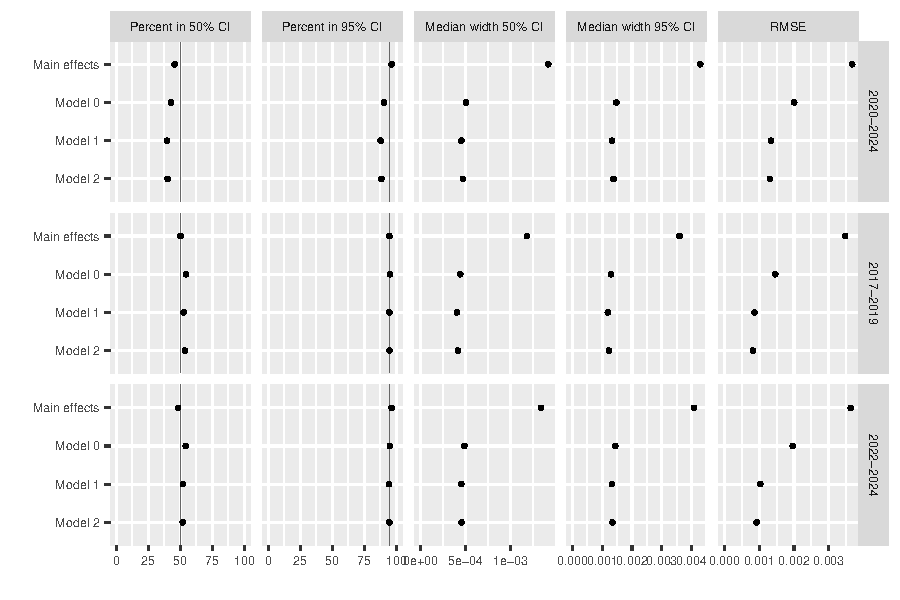
\includegraphics[width = \textwidth]{figures/fig_heldback}
  \centering
  \caption{Some heldback data results}
    \label{fig:heldback}  
\end{figure}

\section{{\color{magenta} Results on Estimates and Forecasts}}
\subsection{Estimates and Forecasts of Internal Migration Rates}

We use the second expanded model to forecast internal migration rates for years 2025-2030. {\color{yellow}Forecasting is done using the R package \texttt{bage}. Internally, \texttt{bage} forecasts the highest-level time-varying terms ($\alpha_t^{\text{time}}$, $\kappa_t^{\text{time}}$,  $\beta_{at}^{\text{age:time}}$, $\beta_{it}^{\text{orig:time}}$,
$\beta_{jt}^{\text{dest:time}}$ and $\beta_{ijat}^{\text{orig:dest:age:time}}$), and then combines the results with estimates for the non-time-varying terms to generate values for the remaining unknowns. The calculations are done separately for each of the 1,000 draws from the posterior distribution for the parameter estimates, which allows uncertainty in the estimates to be propagated through to the forecasts.}

 \begin{figure}[ht]
\includegraphics[width = \textwidth]{figures/fig_forecast_london_se}
  \centering
  \caption{Estimates and forecasts of migration rates from London to the South East. The solid lines represent point estimates, and the light bands represent 95\% credible intervals. The red dots represent direct estimates.}\label{fig:forecast_london_se}  
\end{figure}

 \begin{figure}[ht]
\includegraphics[width = \textwidth]{figures/fig_forecast_se_london}
  \centering
  \caption{Estimates and forecasts of migration rates from the South East to London. The solid lines represent point estimates, and the light bands represent 95\% credible intervals. The red dots represent direct estimates.}\label{fig:forecast_se_london}  
\end{figure}

 \begin{figure}[ht]
\includegraphics[width = \textwidth]{figures/fig_forecast_london_ne}
  \centering
  \caption{Estimates and forecasts of migration rates from London to the North East. The solid lines represent point estimates, and the light bands represent 95\% credible intervals. The red dots represent direct estimates.}\label{fig:forecast_london_ne}  
\end{figure}

As an illustration, Figure~\ref{fig:forecast_london_se}, Figure~\ref{fig:forecast_se_london} and Figure~\ref{fig:forecast_london_ne} show, respectively, estimates and forecasts of migration rates from London to the South East, from the South East to London, and from London to the North East. For the first two origin-destination pairs, the migration counts are not sparse. The modeled estimates track the direct estimates well. For the last origin-destination pair, the migration counts are rather sparse. In the observed data, there are 129 cells with zero migration counts from London to the North East. The modeled estimates appear to do a good job of separating signal and noise. In all three figures, the forecasts capture the changes in age profiles over time for each origin-destination pair.

{\color{magenta} Figures~\ref{fig:forecast_od_female} and \ref{fig:forecast_od_male} in Appendix B show forecasts for all origin-destination pairs in 2030.}
\clearpage

\subsection{{\color{magenta}Estimates of Hyper-parameters}}

{\color{magenta} Table~\ref{tab:hyper} shows the point estimates and 95\% credible intervals for the hyper-parameters. Except for $\sigma_{\text{orig:dest}}$, the standard deviation parameters for the interactions are all relatively small, indicating strong regularization. Regarding the two coefficient parameters in the AR2 prior, $\phi_1$ and $\phi_2$, Table~\ref{tab:hyper} only shows their marginal estimates; but, as mentioned in Section~\ref{subsec:priors}, we checked their posterior draws and found that the stationarity conditions for the AR2 prior were satisfied.}

% latex table generated in R 4.6.1 by xtable 1.8-8 package
% Mon Oct 26 17:40:09 2026
\begin{table}[ht]
\centering
\caption{{\color{magenta}Point estimates and 95\% credible intervals} for hyper-parameters} 
\label{tab:hyper}
\begin{tabular}{lp{3.3cm}p{3.3cm}p{3.7cm}}
  \hline
Hyper-parameter & Initial model & First expanded model & Second expanded model \\ 
  \hline
$\sigma_{\text{orig}}$ & 0.5 (0.11, 2.2) & 0.5 (0.12, 2.1) & 0.5 (0.13,   2) \\ 
$\sigma_{\text{dest}}$ & 0.49 (0.13, 2.1) & 0.52 (0.12, 2.1) & 0.53 (0.12, 2.1) \\ 
$\sigma_{\text{age}}$ & 0.036 (0.01, 0.12) & 0.035 (0.0085, 0.12) & 0.034 (0.011, 0.13) \\ 
$\phi_1$ & 0.1 (-0.38, 0.52) & 0.092 (-0.43, 0.55) & 0.094 (-0.43, 0.54) \\ 
$\phi_2$ & 0.011 (-0.45, 0.48) & 0.022 (-0.43, 0.47) & 0.043 (-0.47, 0.49) \\ 
$\sigma_{\text{time}}$ & 0.068 (0.041, 0.11) & 0.069 (0.043, 0.11) & 0.069 (0.041, 0.11) \\ 
$\eta_{\text{time}}$ & 0.016 (0.0012, 0.03) & 0.016 (0.0024, 0.029) & 0.016 (0.0015, 0.03) \\ 
$\sigma_{\text{orig:dest}}$ & 0.56 (0.46, 0.67) & 0.16 (0.041, 0.69) & 0.18 (0.049, 0.74) \\ 
$\sigma_{\text{orig:age}}$ & 0.041 (0.038, 0.043) & 0.038 (0.036, 0.041) & 0.011 (0.0042, 0.026) \\ 
$\sigma_{\text{orig:time}}$ & 0.03 (0.025, 0.035) & 0.03 (0.025, 0.034) & 0.029 (0.025, 0.034) \\ 
$\sigma_{\text{dest:age}}$ & 0.059 (0.056, 0.062) & 0.056 (0.053, 0.06) & 0.043 (0.034, 0.055) \\ 
$\sigma_{\text{dest:time}}$ & 0.027 (0.023, 0.031) & 0.027 (0.023, 0.031) & 0.027 (0.023, 0.031) \\ 
$\sigma_{\text{age:time}}$ & 0.046 (0.044, 0.049) & 0.047 (0.045, 0.05) & 0.048 (0.046, 0.051) \\ 
$\sigma_{\text{age:sex}}$ & 0.021 (0.018, 0.025) & 0.022 (0.018, 0.025) & 0.021 (0.018, 0.025) \\ 
$\sigma_{\text{orig:dest:age}}$ &  & 0.042 (0.041, 0.043) & 0.0043 (0.0011, 0.017) \\ 
$\sigma_{\text{orig:dest:age:sex}}$ &  &  & 0.02 (0.019, 0.021) \\ 
$\sigma_{\text{orig:dest:age:time}}$ &  &  & 0.038 (0.037, 0.039) \\ 
   \hline
\end{tabular}
\end{table}


 \subsection{{\color{magenta}A Sensitivity Analysis}}

 {\color{magenta}Because the rates are our inferential target, we assess whether their estimates and forecasts are sensitive to the prior specification. Specifically, we conduct a sensitivity analysis with respect to the prior scale for the standard deviation parameters. In our main results, all standard deviation parameters have a prior scale of 1. We also considered prior scales of 0.1 and 0.5 and found that the estimates and forecasts of the rates were not sensitive to the choice of prior scale. We illustrate the results in Figures~\ref{fig:sensitivity_female} and \ref{fig:sensitivity_male} in the Appendix C.}


\section{Conclusion}

%Internal migration is important for understanding sub-national population changes, but modeling and forecasting internal migration rates are difficult due to heterogeneity and sparsity in the data. 

%We propose Bayesian models that can deal with heterogeneity and sparsity. We also apply Bayesian model selection and model checking methods, and select a model that can capture complex interactions in the data. The model works well for both estimation and forecasting of internal migration rates.

Modeling internal migration is essential for understanding and preparing for subnational population change. Progress on estimating and forecasting internal migration rates has, however, lagged behind progress on modeling other demographic rates. The task of modeling internal migration involves multiple technical challenges, including large, sparse datasets and enormous heterogeneity across age, sex, region, and time. 

In this paper we develop and apply a Bayesian hierarchical model that copes well with sparsity and heterogeneity. The preferred model is complex, involving two fourth-order interactions. This complexity is, however, necessary to capture important features of the data, such as changes in the age-sex profile of migration between some regions. Moreover the model performs well in forecasting, generating sensible forecasts over 5-year time horizons.

Bayesian models have a bad reputation among applied modelers for being slow. As we illustrate in this paper, however, recent advances in technologies for fast approximation, and careful use of techniques such as marginalization, can make Bayesian methods feasible for a wide range of applications. Fitting our most complex model to a dataset with 170,352 cells takes about one hour. The practical barriers to the use of large Bayesian hierarchical models are disappearing.

\clearpage

\bibliographystyle{apalike}
\bibliography{references}


\newpage

%\appendix

\section*{Appendix}

\subsection*{{\color{magenta}A. More Results on Forecasting}}
{\color{magenta}Figure~\ref{fig:forecast_od_female} and ~\ref{fig:forecast_od_male} present forecasts of migration rates for all origin-destination pairs in 2030, for females and males, respectively.}
 \begin{figure}[ht]
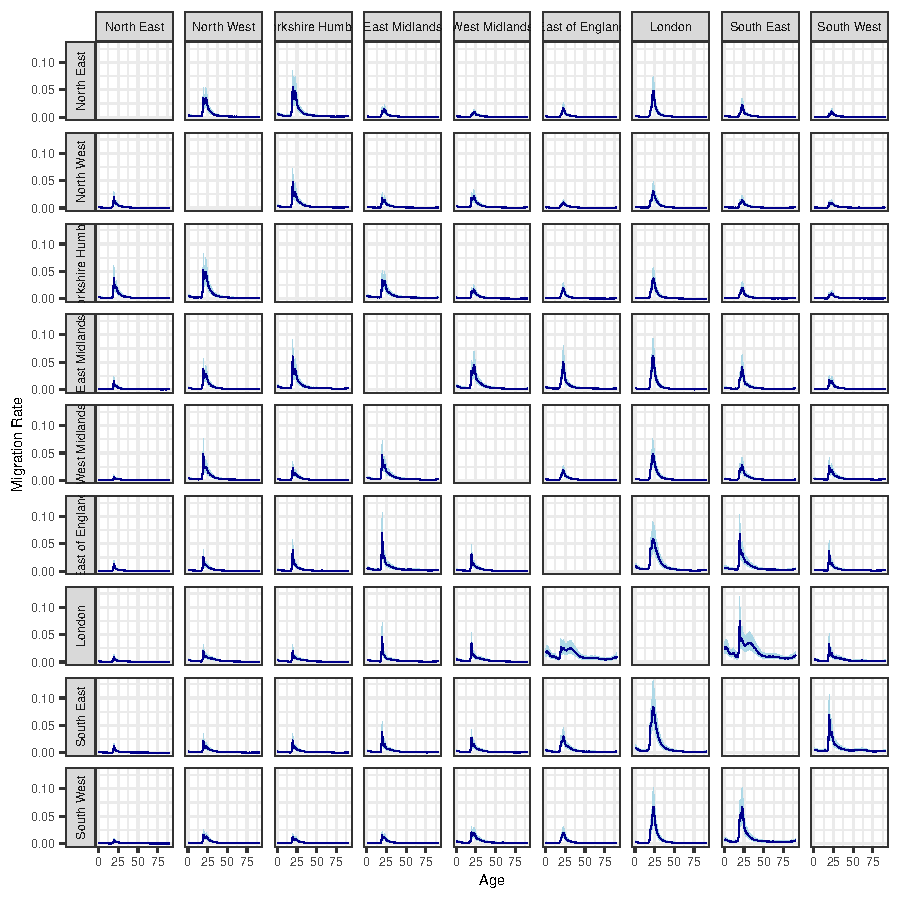
\includegraphics[width = \textwidth]{figures/fig_forecast_od_female}
  \centering
  \caption{Forecasts {\color{magenta}of migration rates} {\color{yellow}for all origins and destinations}{\color{magenta}for all origin-destination pairs}, 2030, females}
    \label{fig:forecast_od_female}  
\end{figure}

  \begin{figure}[ht]
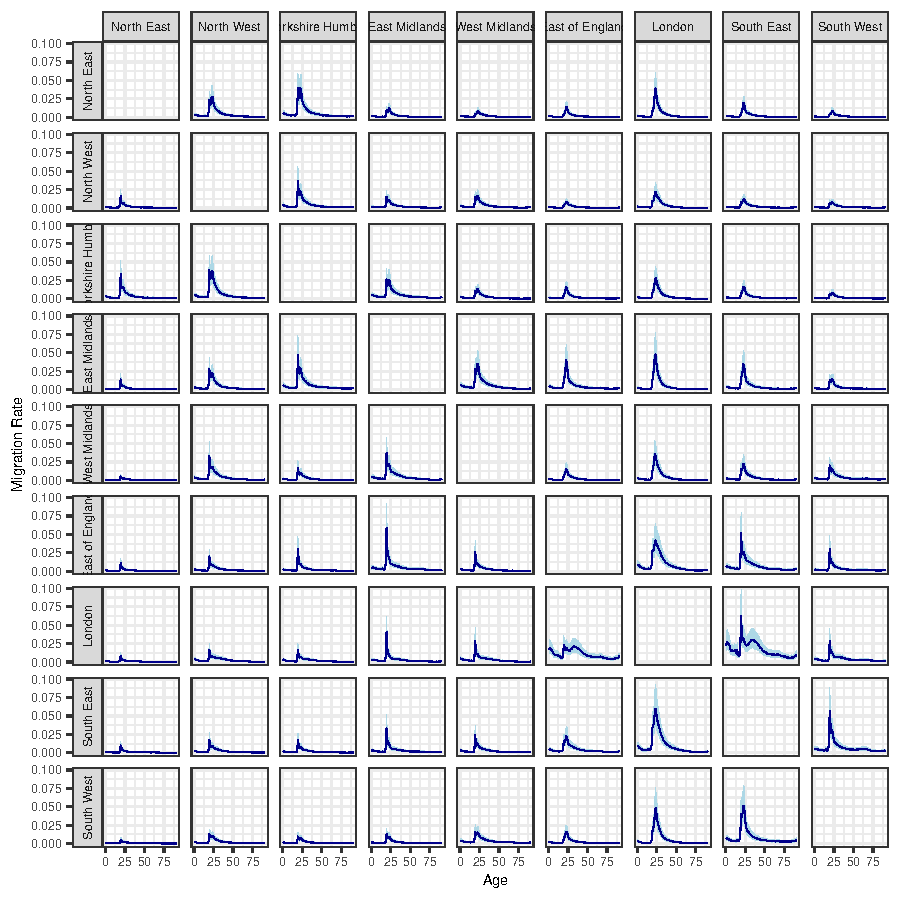
\includegraphics[width = \textwidth]{figures/fig_forecast_od_male}
  \centering
  \caption{Forecasts {\color{magenta}of migration rates} {\color{yellow}for all origins and destinations}{\color{magenta}for all origin-destination pairs}, 2030, males}
    \label{fig:forecast_od_male}  
\end{figure}

\clearpage
\subsection*{{\color{magenta}B. Results on Sensitivity Analysis}}
{\color{magenta}Figures~\ref{fig:sensitivity_female} and ~\ref{fig:sensitivity_male} present estimates and forecasts of migration rates from London to the South East for different prior scale specifications, for females and males, respectively. The results were not sensitive to the choice of prior scale.}

 \begin{figure}[ht]
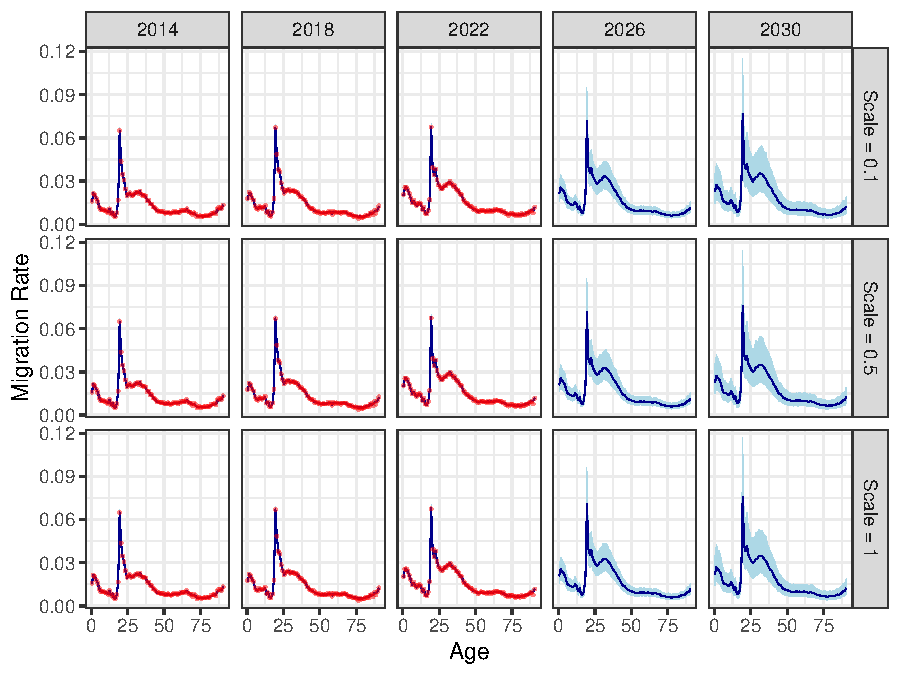
\includegraphics[width = 0.7\textwidth]{figures/fig_sensitivity_all_female}
  \centering
  \caption{{\color{magenta}Estimates and forecasts of female migration rates from London to the South East for different prior scale specifications}}
    \label{fig:sensitivity_female}  
\end{figure}

\begin{figure}[ht]
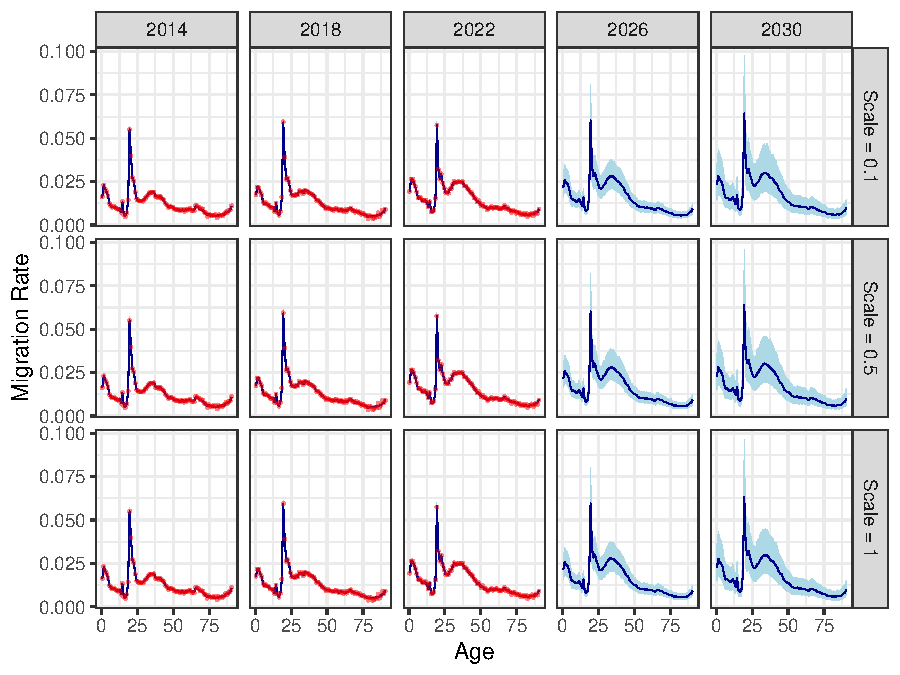
\includegraphics[width = 0.7\textwidth]{figures/fig_sensitivity_all_male}
  \centering
  \caption{{\color{magenta}Estimates and forecasts of male migration rates from London to the South East for different prior scale specifications}}
    \label{fig:sensitivity_male}  
\end{figure}

\end{document}
